\subsubsection{Example Based Super Resolution}
\noindent
En particular, \cite{freeman} propone un parchado de la imagen rescalada a partir
de un conjunto de entrenamiento o diccionario de parches en pares de alta
y baja resolución. Dichos parches permiten construir una imagen con frecuencias
altas que no están en la imagen de entrada con el objetivo de sumar la imagen
original interpolada con las frecuencias altas que buscan mejorar su resolución
al realzar sus detalles. En la Figura \ref{fig:fr_algoritmo} puede observarse de manera específica el algoritmo 
propuesto por \cite{freeman}.

\begin{figure}[H]
    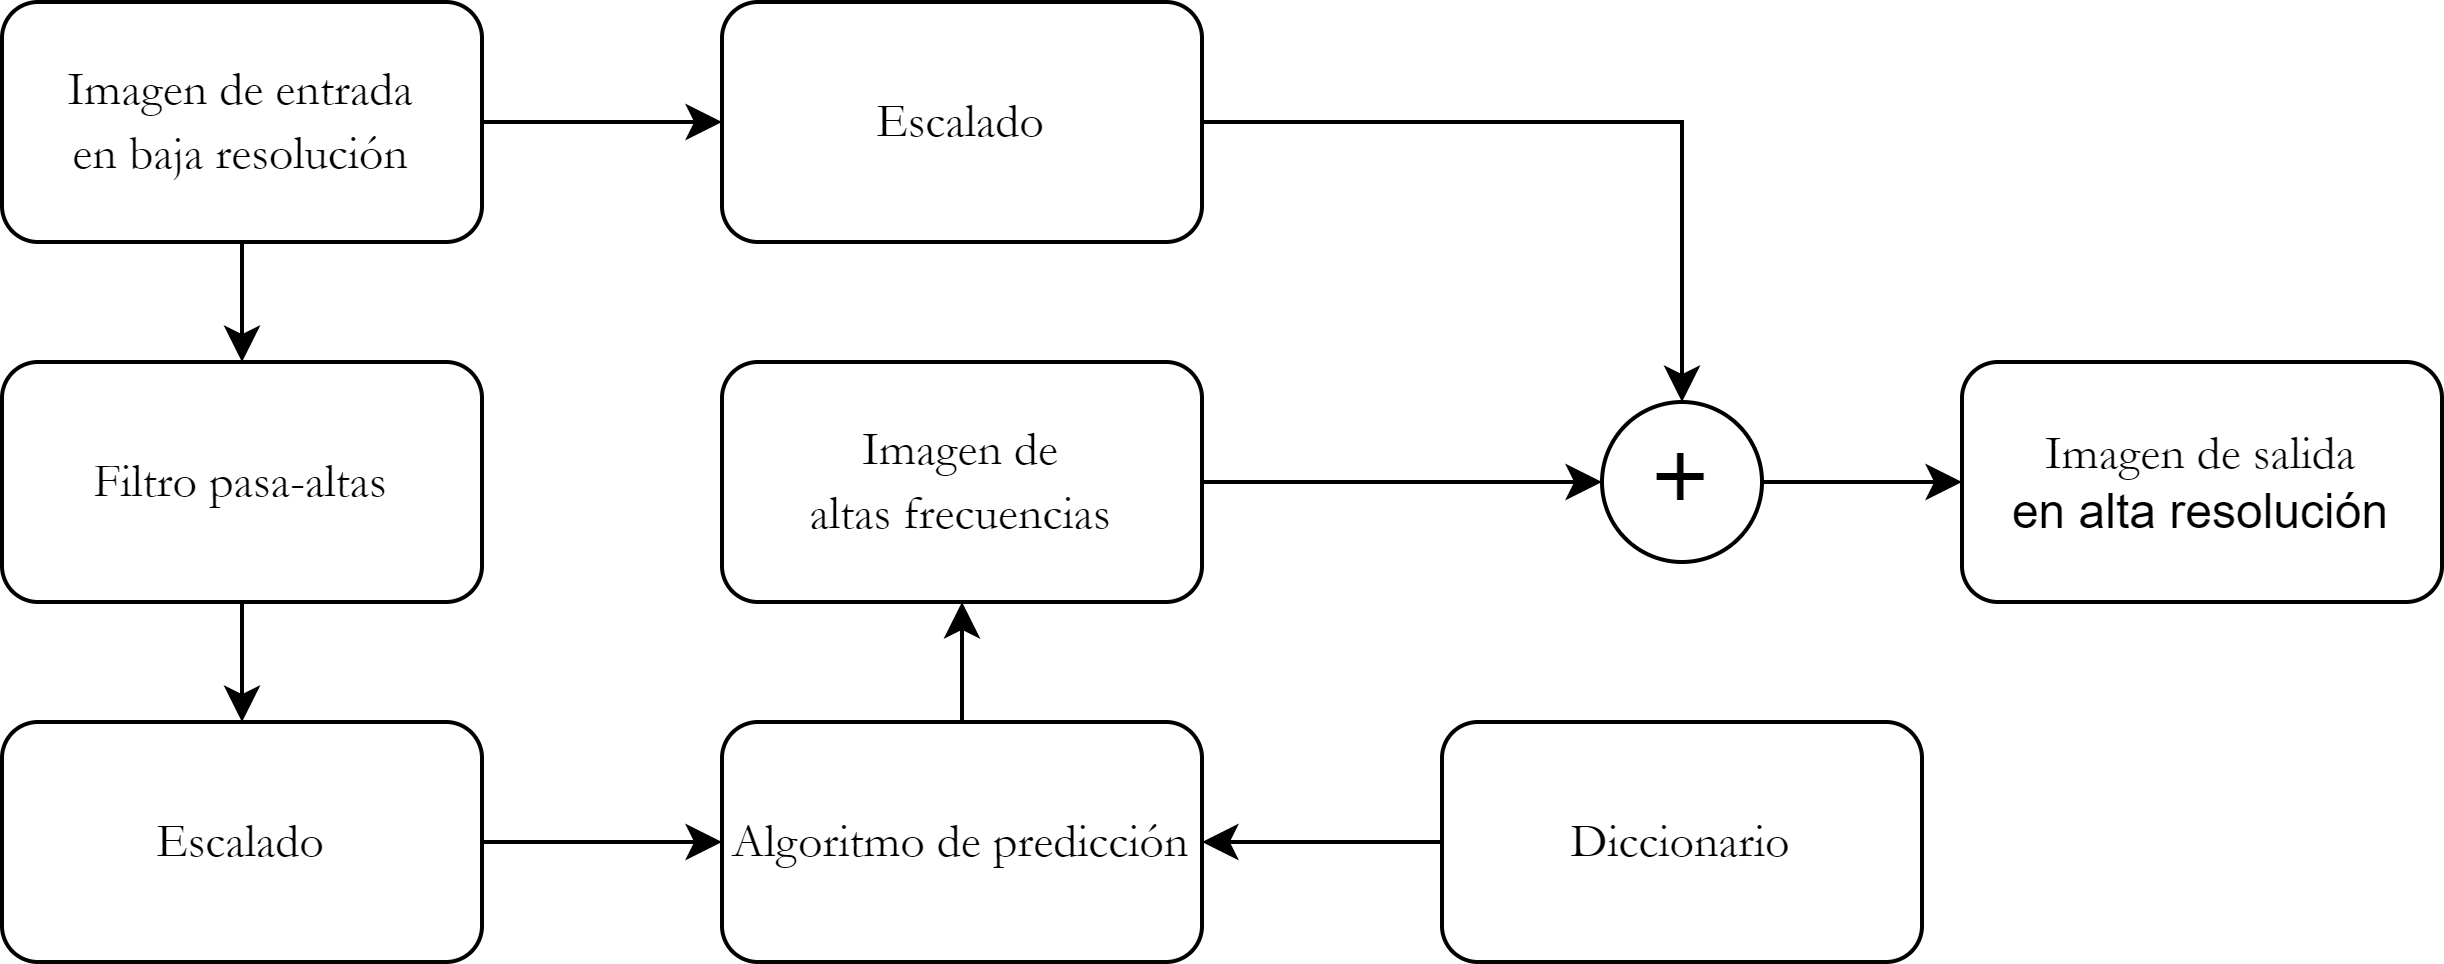
\includegraphics[scale = 0.8]{ fr_algoritmo.png }
    \centering
    \caption{ Algoritmo de súper resolución }
    \label{fig:fr_algoritmo}
\end{figure}

Observe que la imagen de entrada debe pre-porcesarse mediante la aplicación de un 
filtro pasa-altas y el escalado mediante alguna técnica de interpolación. 

